\documentclass[10pt]{beamer}

\usetheme[progressbar=frametitle]{metropolis}
\usepackage{appendixnumberbeamer}

\usepackage{booktabs}
\usepackage{svg}
\usepackage[scale=2]{ccicons}

\usepackage{pgfplots}
\usepgfplotslibrary{dateplot}

\usepackage{xspace}
\newcommand{\themename}{\textbf{\textsc{metropolis}}\xspace}
\usetikzlibrary{positioning}

\title{Computer Architecture and C}
\subtitle{A look beneath}
\date{\today}
\author{Stefan Dennig}
\institute{NewTec GmbH}
% \titlegraphic{\hfill\includegraphics[height=1.5cm]{logo.pdf}}

\begin{document}
\metroset{block=fill}
\maketitle

%\begin{frame}{Table of contents}
%  \setbeamertemplate{section in toc}[sections numbered]
%  \tableofcontents%[hideallsubsections]
%\end{frame}

\section[Intro]{Code Execution}

\begin{frame}[fragile]{CPU Structure}
  \begin{center}
  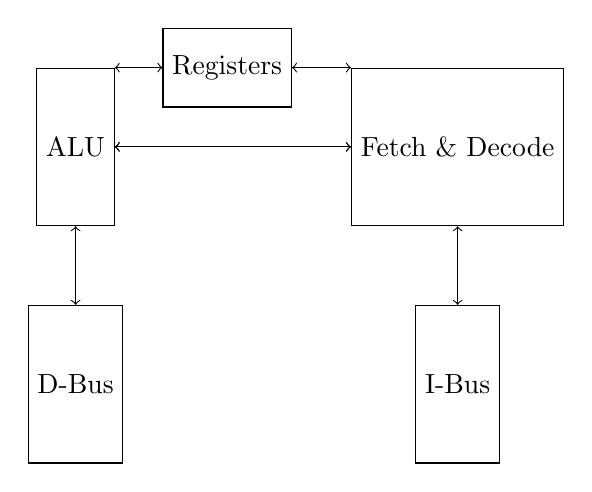
\begin{tikzpicture}

\node [draw, minimum width=0.1cm, minimum height=2cm]  (f_d) {Fetch \& Decode};
\node [draw, minimum width=0.1cm, minimum height=1cm, left=0.75cm of f_d.north west]  (registers) {Registers};
\node [draw, minimum width=0.1cm, minimum height=2cm, left=3cm of f_d]  (alu) {ALU};
\node [draw, minimum width=0.1cm, minimum height=2cm, below=1cm of f_d]  (i_bus) {I-Bus};
\node [draw, minimum width=0.1cm, minimum height=2cm, below=1cm of alu]  (d_bus) {D-Bus};

\draw [<->] (f_d.south) -- (i_bus.north);
\draw [<->] (alu.south) -- (d_bus.north);
\draw [<->] (f_d.west) -- (alu.east);
\draw [<->] (alu.east) -- (f_d.west);

\draw [<->] (alu.north east) -- (registers.west);
\draw [<->] (registers.east) -- (f_d.north west);

\end{tikzpicture}
  \end{center}
\end{frame}

\begin{frame}[fragile]{Von Neumann Architektur}
  \begin{center}
  \input{von_neumann_architecture.tex}
  \end{center}
\end{frame}

\begin{frame}[fragile]{Example implementation}
  \begin{center}
  \input{von_neumann_architecture_implementation.tex}
  \end{center}
\end{frame}

\begin{frame}[fragile]{Execute Instruction}
\begin{itemize}
  \item Fetch at Program Counter using I-Bus
  \item Decode Instruction
  \item Access Operands
  \item Execute
\end{itemize}

\begin{block}{Example}
  mov r1,r2
\end{block}

\begin{alertblock}{Instruction fetches}
 Instruction fetches may stall the CPU.
\end{alertblock}
\end{frame}

\begin{frame}[fragile]{Load Instruction}
\begin{itemize}
  \item Fetch at Program Counter using I-Bus
  \item Decode Instruction
  \item Access Operands
  \item Read data from RAM
\end{itemize}

\begin{block}{Example}
  ldr r1, [r2]
\end{block}

\begin{alertblock}{Memory Writes}
  Memory Reads may stall the CPU
\end{alertblock}

\end{frame}


\begin{frame}[fragile]{Store Instruction}
\begin{itemize}
  \item Fetch at Program Counter using I-Bus
  \item Decode Instruction
  \item Access Operands
  \item Write Data to Store Buffer
\end{itemize}

\begin{block}{Example}
  str r1, [r2]
\end{block}

\begin{alertblock}{Memory Writes}
  Memory Writes may not be executed immediately.
\end{alertblock}

\end{frame}

\begin{frame}[fragile]{Reason?}
\begin{itemize}
  \item RAM/ROM can be slower than fcpu
  \item Access may needs longer Time
  \item Different Bus master Accesses same Bus
\end{itemize}
\end{frame}

\begin{frame}[fragile]{Bus}
  \begin{columns}[T,onlytextwidth]
    \column{0.33\textwidth}
    Master Interface
    \begin{itemize}
      \item Read Request
      \item Write Request
      \item Address Based
      \item Word Size
    \end{itemize}
    \column{0.33\textwidth}
    Slave Interfaces
    \begin{itemize}
      \item Read Response 
      \item Write Response
      \item Mapped on Address Range
      \item Word Size
    \end{itemize}
    \column{0.33\textwidth}
    Bus as Multiplexer
    \begin{itemize}
      \item Maps Requests for Slave Address Range to Slave
      \item Multiple Channels possible (Multi Master)
    \end{itemize}
  \end{columns}
\begin{center}
  \vspace{2cm}
  \href{https://www.google.com/url?sa=t&source=web&rct=j&opi=89978449&url=https://www.st.com/resource/en/reference_manual/rm0454-stm32g0x0-advanced-armbased-32bit-mcus-stmicroelectronics.pdf&ved=2ahUKEwi60-Sj-JyRAxUc_7sIHQfdIJwQFnoECAwQAQ&usg=AOvVaw3lSwbTb5IyN9LnayPYfHpf}{STM32g070 Reference Manual}
\end{center}
\end{frame}

\end{document}
